\documentclass{tudelft-report}
\usepackage{indentfirst}


% 1)Translates MATLAB code:
\usepackage[framed,numbered,autolinebreaks,useliterate]{mcode}
% enclose the MATLAB code by using begin/end{lstlisting}

% 2)Multiple figures on one page
\usepackage{float}
\usepackage[caption = false]{subfig}
\usepackage{fancyvrb}
\usepackage{graphicx}
% 3)


\begin{document}

%% Use Roman numerals for the page numbers of the title pages and table of
%% contents.
\frontmatter

\title[Implementation of Election in Asynchronous Complete Networks]{Distributed Algorithms}
\author{Jo\~ao Almeida\\Manuel Ribeiro}
\affiliation{Faculty of Electrical Engineering, Mathematics and Computer Science}

%coverimage{cover.jpg}
%\makecover[backboxheight = 2.64in]


%% Include an optional title page.
\begin{titlepage}

\begin{center}

%% Insert the TU Delft logo at the bottom of the page.
\begin{tikzpicture}[remember picture,overlay]
    \node at (current page.south)[anchor=south,inner sep=0pt]{
        
\includegraphics{cover/logo}
    };
\end{tikzpicture}

%% Extra whitespace at the top.
\vspace*{2\bigskipamount}

%% Print the title in cyan.
{\makeatletter
\titlestyle\color{tudelft-cyan}\Huge\@title
\makeatother}

%% Print the optional subtitle in black.
{\makeatletter
\ifx\@subtitle\undefined\else
    \bigskip
    \titlefont\titleshape\LARGE\@subtitle
\fi
\makeatother}

\bigskip
\bigskip

by
%door

\bigskip
\bigskip

%% Print the name of the author.
{\makeatletter
\titlefont\Large\bfseries\@author
\makeatother}

\vfill

\bigskip
\bigskip

\bigskip
\bigskip
\vfill

\end{center}

\end{titlepage}





%% Use Arabic numerals for the page numbers of the chapters.
\mainmatter

\section*{Tests Introduction}

	\vspace{10pt}

	\indent To guarantee the quality of our implementation we ran multiple tests, a summary of those tests is present in Table \ref{tab:testtable}. To ensure the algorithm was implemented correctly, information regarding the state of the processes was printed during the execution of the algorithm. All these tests are explained in the section \textit{Detailed Tests}.

	For each test we measured a series of parameters to evaluate the output of the algorithm. The parameters are:

	\begin{itemize}
		\item{\textbf{Number of Level Increases:}} Sum of the \textit{Levels} of all processes at the end of execution. 
		\item{\textbf{Number of Messages:}} Number of all messages of the implementation.
		\item{\textbf{Number of Captures:}} Number of \textit{Captures} that were successful, measured by the ordinary processes.
		\item{\textbf{Number of Kill messages:}} Number of messages sent by ordinary processes to \textit{Kill} their previous owner.
		\item{\textbf{Number of Acknowledgment messages:}} Number of \textit{Acknowledgment} messages sent for each \textit{kill} or \textit{Capture} messages.
		\item{\textbf{Number of Capture/Level Discrepancies:}} The difference between the number of \textit{Captures} and number of \textit{Level Increases}.

	\end{itemize}

	\begin{table}[h] 
		\centering
		\resizebox{\textwidth}{!}{%
		\begin{tabular}{|c|c|c|c|c|c|c|c|c|}
		\hline 
		Test \# & \# Machines & Total \# Processes & \#Level increases & \# Captures & \# Kills & \# Acks & \# Messages & \begin{tabular}[c]{@{}c@{}}\#Capture/Level \\ Discrepancies\end{tabular} \\ \hline
		1 & 1 & 2 & 1 & 1 & 0 & 1 & 2 & 0 \\ \hline
		2 & 1 & 5 & 4 & 4 & 0 & 4 & 8 & 0 \\ \hline
		3 & 2 & 10 & 9 & 9 & 0 & 9 & 18 & 0 \\ \hline
		4 & 1 & 10 & 13 & 13 & 3 & 16 & 33 & 0 \\ \hline
		5 & 1 & 20 & 30 & 30 & 10 & 40 & 93 & 0 \\ \hline
		6 & 1 & 50 & 65 & 65 & 15 & 79 & 163 & 1 \\ \hline
		7 & 1 & 100 & 151 & 151 & 51 & 199 & 423 & 3 \\ \hline
		8 & 1 & 250 & 421 & 421 & 171 & 589 & 1396 & 3 \\ \hline
		9 & 1 & 500 & 773 & 773 & 274 & 1040 & 2375 & 7 \\ \hline 
		10 & 1 & 750 & 1354 & 1354 & 604 & 1947 & 4556 & 11 \\ \hline
		\end{tabular}
		}
		\caption{Tests summary}\label{tab:testtable}
	\end{table}

	In theory the formula $\#ACKS = \#KILLS+\#CAPTURES$ should be respected for all runs of the algorithm, however for larger tests there is a discrepancy in this formula. This results from a known problem of synchronization, some of these captures do not result in a level increase for the candidate because it is killed before receiving the acknowledgment. This acknowledgment arrives later, however it is ignored, as the candidate is already dead. So this way the number of acknowledgments respects: $\#ACKS = \#KILLS+\#CAPTURES-\#DISCREPANCIES$.
	
	\newpage


\section*{Detailed Tests}		

	\vspace{10pt}

	\begin{Verbatim}[commandchars=\\\{\},codes={\catcode`$=3\catcode`_=8},frame=single,label=Test 1 output]
[INFO]	  	Connections Ready
[Process: 1]	[C]	Is now a Candidate.
[Process: 2]	[O]	Captured by Candidate Process: 1.
\textcolor{red}{[Process: 1]	[C]	Elected!!} 
[Process: 1]	[C]	Level = 2. Times Captured = 0. Acks = 1.
[Process: 2]	[C]	Level = 1. Times Captured = 1. Acks = 0.
[INFO]		
Level Sum - Number of Processes = 1.	
Captures Sum = 1	
Total Kills = 0	
Total Acks = 1
Missed captures: 0
	\end{Verbatim}

	\vspace{10pt}

	In this example , \textit{Test 1}, two processes are trying to get elected. Process 1 is the first candidate and captures Process 2 immediately, making itself the elected process. The '\textit{Level Sum - Number of Processes}' is equal to the '\textit{Captures Sum}', which proves the correctness of the algorithm for two processes.

	\vspace{10pt}
	
	\begin{Verbatim}[commandchars=\\\{\},codes={\catcode`$=3\catcode`_=8},frame=single,label=Test 4 output]
[INFO]	  			Connections Ready
[Process: 9]	[C]	Is now a Candidate.
[Process: 1]	[C]	Is now a Candidate.
[Process: 7]	[C]	Is now a Candidate.
[Process: 5]	[C]	Is now a Candidate.
[Process: 4]	[C]	Is now a Candidate.
[Process: 2]	[C]	Is now a Candidate.
[Process: 8]	[C]	Is now a Candidate.
[Process: 3]	[C]	Is now a Candidate.
[Process: 10]       [C]	Is now a Candidate.
[Process: 6]	[C]	Is now a Candidate.
[Process: 5]	[O]	Captured by Candidate Process: 4.
[Process: 8]	[O]	Captured by Candidate Process: 1.
[Process: 9]	[O]	Captured by Candidate Process: 2.
[Process: 2]	[O]	Captured by Candidate Process: 5.
[Process: 4]	[O]	Captured by Candidate Process: 9.
[Process: 6]	[O]	Captured by Candidate Process: 7.
[Process: 3]	[O]	Captured by Candidate Process: 4.
[Process: 10]       [O]	Captured by Candidate Process: 7.
[Process: 1]	[O]	Captured by Candidate Process: 2.
[Process: 1]	[C]	Was Killed
[Process: 1]	[C]	Received a kill Message, but was already killed.
[Process: 8]	[O]	Captured by Candidate Process: 7.
[Process: 1]	[C]	Received a kill Message, but was already killed.
[Process: 1]	[O]	Captured by Candidate Process: 7.
[Process: 2]	[C]	Was Killed
[Process: 5]	[O]	Captured by Candidate Process: 7.
[Process: 4]	[C]	Was Killed
[Process: 2]	[O]	Captured by Candidate Process: 7.
[Process: 5]	[C]	Was Killed
[Process: 9]	[O]	Captured by Candidate Process: 7.
[Process: 2]	[C]	Received a kill Message, but was already killed.
[Process: 4]	[O]	Captured by Candidate Process: 7.
[Process: 9]	[C]	Was Killed
[Process: 3]	[O]	Captured by Candidate Process: 7.
[Process: 4]	[C]	Received a kill Message, but was already killed.
\textcolor{red}{[Process: 7]	[C]	Elected!!}
[Process: 1]	[C]	Level = 2. Times Captured = 2. Acks = 4.
[Process: 2]	[C]	Level = 3. Times Captured = 2. Acks = 4.
[Process: 3]	[C]	Level = 1. Times Captured = 2. Acks = 0.
[Process: 4]	[C]	Level = 3. Times Captured = 2. Acks = 4.
[Process: 5]	[C]	Level = 2. Times Captured = 2. Acks = 2.
[Process: 6]	[C]	Level = 1. Times Captured = 1. Acks = 0.
[Process: 7]	[C]	Level = 10. Times Captured = 0. Acks = 9.
[Process: 8]	[C]	Level = 1. Times Captured = 2. Acks = 0.
[Process: 9]	[C]	Level = 2. Times Captured = 2. Acks = 2.
[Process: 10]       [C]	Level = 1. Times Captured = 1. Acks = 0.
[INFO]		
Level Sum - Number of Processes = 16	
Captures Sum = 16
Total Kills = 9	
Total Acks = 25
Missed captures: 0
	\end{Verbatim}

	\vspace{10pt}

	With this example from \textit{Test 4} we want to prove that even if all candidates start the election at the same time, the algorithm still works as expected.

\newpage
\section*{Conclusion}

Our implementation worked exactly as expected on small and medium size tests, on larger tests, more than 50 processes, the algorithm still elected one process correctly. In those large tests there were some small synchronization problems that can be easily explained by the large number of processes trying to communicate with each other at the same time.

To guarantee that our implementation has the message complexity of the algorithm we the number of messages and the evolution of the $ n log(n)$ function. In Figure \ref{ComplexityAnalysis} you can see clearly that the two lines have the same evolution. The axis are in a logarithmic scale that allows us to represent both functions as almost straight lines.

\begin{figure}[h] \centering
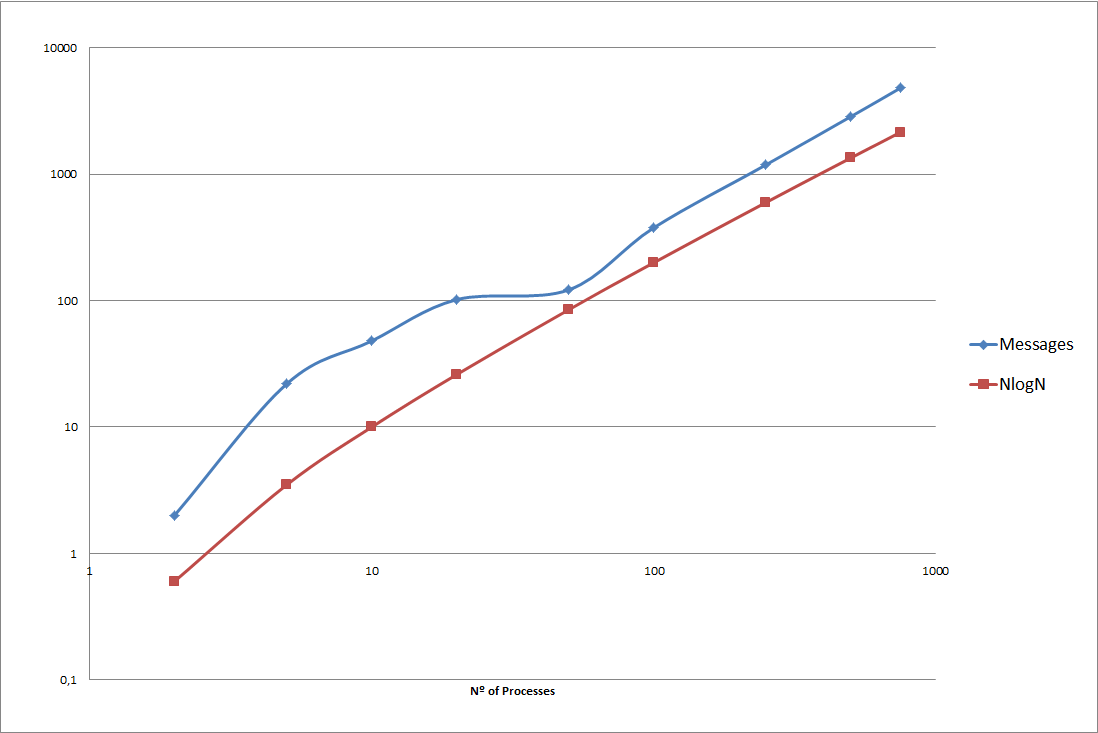
\includegraphics[scale=0.5]{ComplexityAnalysisPlot}\caption{Complexity Analisys of the implementation} \label{ComplexityAnalysis}
\end{figure}
	



\end{document}

